%--------------------
% Packages
% -------------------
\documentclass[11pt,a4paper]{article}
\usepackage[utf8]{inputenc}
\usepackage[T1]{fontenc}
\usepackage{outlines}
%\usepackage{gentium}
\usepackage{mathptmx} % Use Times Font
\usepackage{algorithmic}
\usepackage{booktabs}

\usepackage[pdftex]{graphicx} % Required for including pictures
\usepackage[pdftex,linkcolor=black,pdfborder={0 0 0}]{hyperref} % Format links for pdf
\usepackage{calc} % To reset the counter in the document after title page
\usepackage{enumitem} % Includes lists

\frenchspacing % No double spacing between sentences
\linespread{1.2} % Set linespace
\usepackage[a4paper, margin=2cm]{geometry} %margins
\usepackage{subcaption}

\usepackage[all]{nowidow} % Tries to remove widows
\usepackage[protrusion=true,expansion=true]{microtype} % Improves typography, load after fontpackage is selected
\usepackage{csquotes}
\usepackage[style=verbose-ibid,backend=bibtex]{biblatex}
\bibliography{bibliography}

%-----------------------
% Set pdf information and add title, fill in the fields
%-----------------------
\hypersetup{ 	
pdfsubject = {},
pdftitle = {INNS Open Assessment},
pdfauthor = {}
}

\title{INNS COM00029H Open Assessment}

\author{Y3843100}

\date{\today}
%-----------------------
% Begin document
%-----------------------
\begin{document}
% ! ============
% ! Terminology
% ! ============
% CTG - Cardiotocogram
% FHR - fetal heart rate
% STM - short term variability::  beat-to-beat differences between consecutive heart beats
% LTM - long term variability:: variations in the interval length over N R-R intervals
% R-R interval - beat-to-beat time.


\maketitle


\section{[20 marks] Discussion of architectures.}
\label{sec:discussion}
This section should:
\begin{outline}
  \1 describe (briefly) the data you have, and how much there is of it.
  \1 identify the type of problem
  \1 identify which classes of architectures would be suitable
  \1 give a brief discussion of the technical features of the architectures, and the advantages and disadvantages of each
  \1 state which class of architecture you are going to use and justify your choice, relating the characteristics of the problem to the advantages/disadvantages of the architecture.
\end{outline}

To do this you might need to:
\begin{outline}
  \1 do some preliminary experiments with simple versions of the architecture to get a feel for what will work
  \1 do some exploratory data analysis to see what the characteristics of the data are
  \1 consider the principles involved and relate them to the problem.
\end{outline}

\paragraph{}
The dataset contains fetal cardiotocograms (CTGs) from 2126 patients each of which has 21 different recorded features (input variables). The CTGs have been annotated by three expert obstetricians creating two categories of classes \autocite{Campos:2000}. One is a 10 tuple with respect to the fetal heart rate FHR patterns and the other is a three tuple regarding fetal state. This gives us two supervised classification problems with respectively 10 and 3 distinct classes. Neural Network architectures that can handle classification problems need to have appropriate activation functions and the ability to specify the targets (outputs) as a finite set of discrete classes. We will discuss \textbf{three} different conceptual models with respect to their ability to be configured for classifying our high dimensional CTG dataset.

\subsubsection{Perceptron}
The \textit{perceptron} is a basic network structure in which our output class \(y\) is determined by a weighted sum of our inputs \(X\) that is evaluated against some hard limit (threshold or activation function) \(y = H(\sum_{i}^{X} x_i w_i)\). Both the advantages and disadvantages of the perceptron are in its simplicity. On one hand we have intuitive behaviour in the fact that the perceptron finds a line that bipartitions our data space, but on the other we are limited only to linearly separable classes. Furthermore a perceptron can perform only binary classification or at best \textit{one-vs-many}.

\subsubsection{Multi-Layer Perceptron MLP networks}
The shortcomings of the single perceptron are addressed by its orchestrated counterpart, the multi-layer perceptron \textit{MLP}. The three main differences as highlighted by Haykin \autocite{Haykin1998} are:

\begin{outline}
  \1 neuron activation functions are differentiable (sigmoid functions are often chosen), unlike the hard limits we had before
  \1 between our input and output layers we construct one or more \textit{hidden layers} containing one or more neurons
  \1 the input, output and hidden neurons are highly connected
\end{outline}

% ? Argument about we cannot add more datapoints therefore we will have to find the best network.
By composing neurons together we can learn more complex patterns at the expense of more complicated learning rules. The benefit of MLPs is that that they can approximate virtually any function provided there is enough data. The disadvantages of using MLPs come from the fact that they are prone to overfitting on high dimensional data and they do not necessarily have a simple intuitive meaning as the perceptron classifier. We can theoretically use MLPs for our two classification problems as we can specify the number of output neurons to be three and ten respectively. An issue arrises with what network structure would be viable to capture the properties of our high dimensional data. 

%Due to the continuous activation function, neurons in MLPs are able to propagate their weights forward in the network and influence subsequent neurons. Because we have a supervised problem, we can define the notion of error \(e\) as the difference between the true classes \(d\) and our network's outputs. The error at each neuron is \(E = \frac{1}{2}e^{2}\). Training the MLP is a matter of minimising the error with respect to the weights which is often done by a gradient descent algorithm. An issue arrises with the fact that the error is known only at the output layer. To correctly adjust the weights on each neuron, we use a backpropagation method to communicate how weight changes affect the error. Knowing the mechanisms involved in using MLPs we can determine two issues: what network structure is viable for our problems and how can we learn the weights of each neuron now that they are connected?

\subsubsection{Radial Basis Function RBF networks}
RBF networks are a single hidden layer MLP where Euclidean distance between the inputs and some point in space associated with the neuron's centre is computed instead of linear activation function. More specifically, the hidden layers calculate a radially-symmetric function (usually a Gaussian) from the inputs \(f_i(x) = \exp \left(-\frac{{\mid x - c_i \mid}^2}{2 \sigma^2} \right) \) where \(c_i\) is the centre for neuron \(i\). The outputs are the weighted sums of the different basis functions in the hidden layer.
RBF networks classify new data points by associating them to the closest \(c_i\). The benefit of this architecture is that it is often faster to train compared to MLPs, but a substantial drawback is that they struggle with generalising outside of the margins of the training data. But an argument can be made that for our specific task, if we get new patient data that has low response for all of our current classes, that is a potential indicator of an anomaly that would require further investigation.

\subsection{Deep Learning Neural Networks}
%TODO: We can use more complicated architectures but with 2126 datapoints we will be risking overfitting.

\paragraph{}
In the choice of an architecture it is important to look at the data itself. Our data does not appear to be linearly separable and our task is to discriminate between all the distinct classes, therefore we rule out the perceptron as a viable architecture.
MLP and RBF are theoretically viable for both of our classification problems. They both allow for supervised multiclass classification problems and they can solve non-linearly separable problems. Because of our argument that low response from the RBF network is a useful indicator for an anomaly, we will still consider RBFs in this experiment. The severity of the disadvantages for MLP models can be lessened by paying close attention to the meaning of the data and incrementally explore different network structures, applying Occam's razor as a prerequisite. Because of this reasoning, we will empirically compare different MLP and RBF networks for our two classification problems.

%We will assume that the goal of such a classification tool is to be a good predictor of FHR anomalies even if 


% The severity of the disadvantages of the two architectures can be lessened by paying close attention to the meaning of data and by incrementally  .After further investigation of the semantic meaning of the we will empirically compare the two networks with different formulation of our problem. %TODO: revisit this after you know which algorithms we're using exactly.

\section{[40 marks] Creation and application of neural networks.}
\label{sec:creation}
This section should
\begin{outline}
  \1 Describe the chosen inputs to (and outputs from) the networks.
  \1 Describe how the data you started with have been preprocessed.
  \1 Give sufficient detail for someone else to process a new batch of data for use with the final trained network.
  \1 State which training algorithm you selected, and explain how you selected that training algorithm. For this training algorithm, give sufficient detail to enable someone to use the same training algorithm in exactly the same way. This does NOT mean (for example) describing gradient descent in great detail. It DOES mean giving any parameters, initialisation, etc, even if they are the toolbox defaults.
  \1 Explain the process you went through in making the selection of the final architecture, for example, the number of neurons or the number of layers to use.
\end{outline}

To do this you might need to:
\begin{outline}
  \1 Test of one or more networks to demonstrate the effect of different preprocessing choices on the performance of the network.
  \1 Try different training algorithms on one or more networks to compare performance.
  \1 Evaluate a number of networks, and record details of their structures and how they performed. You may summarise repeated tests of the same structure. 
\end{outline}
%Todo: Describe the chosen inputs to (and outputs from) the networks.
%The total set of inputs has been predefined 
\paragraph{}
A crucial observation for our classification problems is to note that classifying biological anomalies is naturally going to mean our classes are unbalanced. This is the case for both the FHR patterns and the fetal state problems (fig. \ref{fig:ClassHistograms}). To mitigate this, we use a simple oversampling method that replicates data from our underrepresented cases until they match the most common class. This method does not give us any new knowledge about the problems, but by scaling the data we take a step towards unbiased estimations when looking at the misclassification rates. We also one-hot encode our classes for use with MATLAB's \texttt{patternnet}.

\begin{figure}[htb]
  \centering
  \begin{subfigure}[b]{0.48\textwidth}
    \centering
    \includegraphics[width=\textwidth]{figures/CLASS_HIST.png}
  \end{subfigure}
  ~
  \begin{subfigure}[b]{0.48\textwidth}
    \centering
    \includegraphics[width=\textwidth]{figures/NSP_HIST.png}
  \end{subfigure}
  \caption{class distributions}
  \label{fig:ClassHistograms}
\end{figure}

\paragraph{}
Noise reduction by high frequency noise and FHR spike removal has been done by the original researchers, but plotting the correlation and distributions of the features reveals further preprocessing is required \ref{fig:plotmatrixX}. Unsurprisingly, we observe the mean, mode and median are highly correlated. We keep only the median as a feature importance analysis (pairwise comparison of the mutual information of each feature and the class \(I(\boldsymbol{X},Y)\) in search of redundancy \autocite{FeatureImportance}) reveals that it has the highest predictive capabilities. It is important to note that the analysis (fig \textbf{insert feature importance fig}) also confirms that the features with highest predictive capabilities are the variance of the CTGs, tendency and the ones related to heart rate accelerations and decelerations. Subsequently we deal with the skewed distributions and non regularised parameters by looking into normalising the data. An empirical test reviews that \((\mu = 0, \sigma^2 = 1)\) regularisation surpasses \([-1;1]\) normalisation performance.

\begin{figure}[htb]{0.48\textwidth}
  \centering
    \centering
    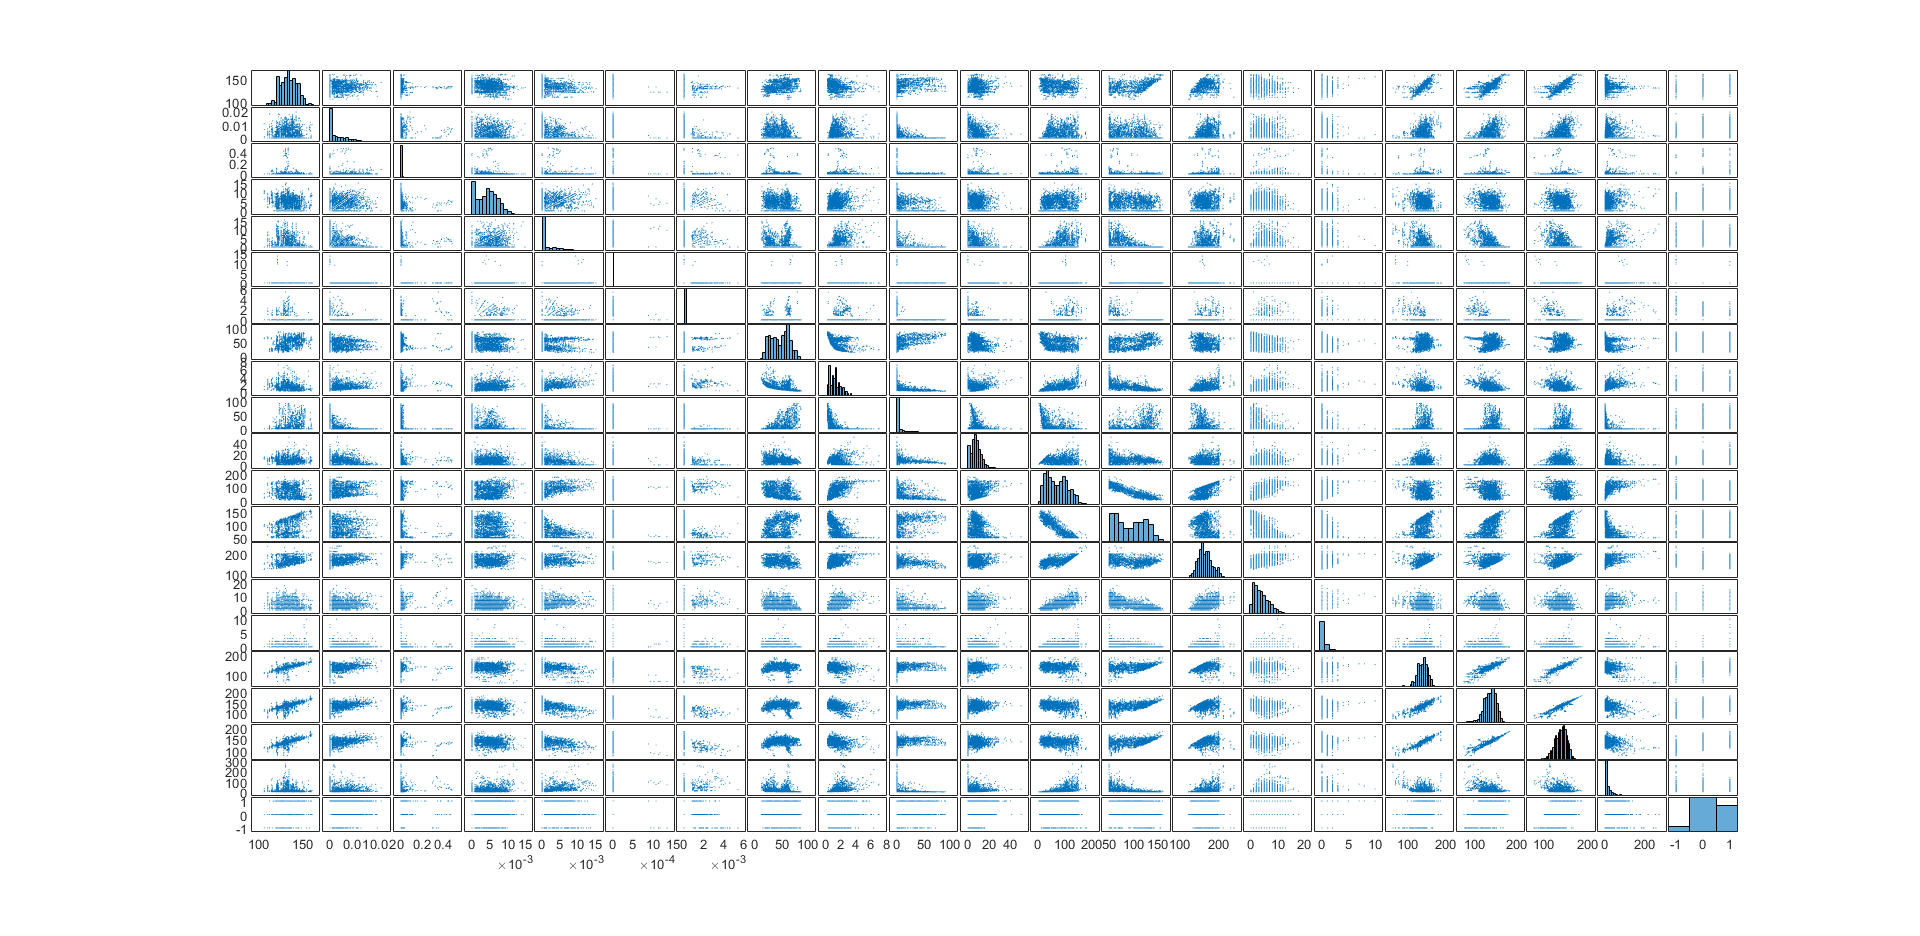
\includegraphics[width=\textwidth]{figures/plotmatrix_X.png}
  \label{fig:plotmatrixX}
\end{figure}

\paragraph{what you need to run this NN}
We disregard training algorithms that compute the Jacobian as they require the network to use a mean-squared error \textit{MSE} loss function, which is not appropriate for our tasks (elaboration on choice of loss functions can be found in section \ref{sec:results}). An empirical comparison of different training algorithms for a network with a single hidden layer with \(N = \{10,15,20,25,30,35,40,45,50\}\) neurons can be seen in figure \ref{fig:algoCompare}. It appears that the family of conjugate gradient backpropagation \textit{CGB} (traincgb, traincgp and traincgf) achieve the best trade-off between performance and training time. At a glance, the results of CGB with Powell-Beale restarts (traincgb) appears to be the most consistent (least noisy) and therefore we will chose it as a training algorithm. The initialisation parameters for traincgb are selected via a Nguyen-Widrow \autocite{NetParamInit} algorithm, which evenly distributes the weights and biases for the active regions across neurons. CGB also does not use a fixed learning rate, but calculates the learning step at each iteration. All the initialisation parameters can be seen in table \ref{tab:InitParams}.

% preprocessing, zero mean and unit variance regularisation for features, one hot encoding for labels and oversampling for both
% activation functions tansigmoid
% training algorithm
% learning rate, initialisation weights
% dataset split, function and ratios
\begin{figure}[htb]
  \centering
  \begin{subfigure}[b]{0.48\textwidth}
    \centering
    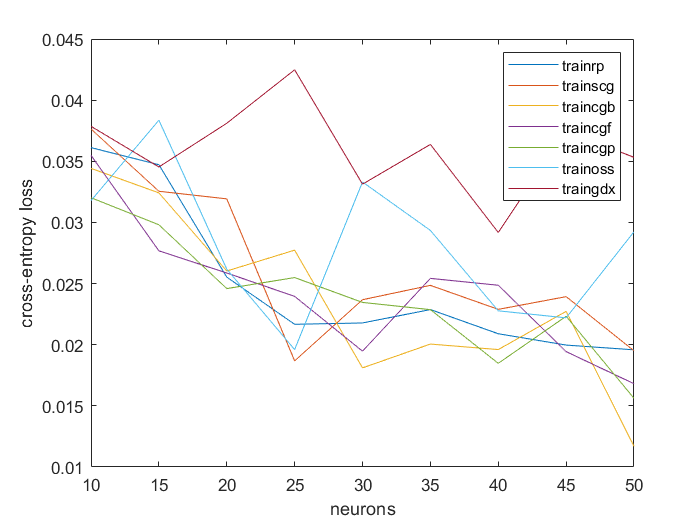
\includegraphics[width=\textwidth]{figures/traininng_algo_comparison_CE.png}
  \end{subfigure}
  ~
  \begin{subfigure}[b]{0.48\textwidth}
    \centering
    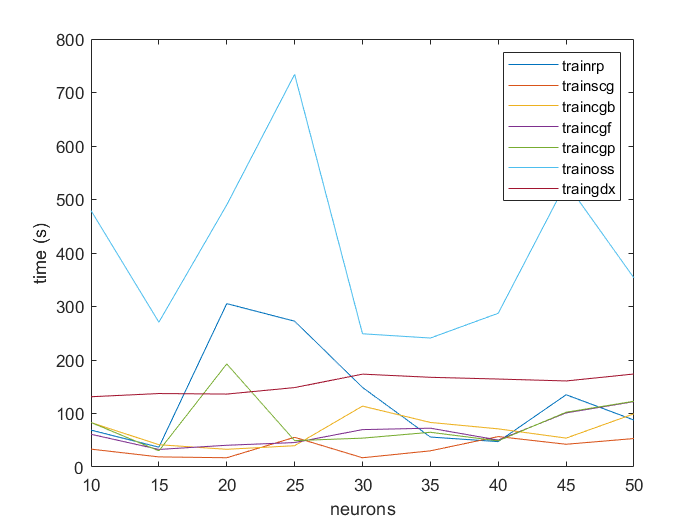
\includegraphics[width=\textwidth]{figures/traininng_algo_comparison_time.png}
  \end{subfigure}
  \caption{CE loss and training time for different training algorithms}
  \label{fig:algoCompare}
\end{figure}

\begin{table}[]
  \begin{tabular}{@{}llllllllllll@{}}
  \toprule
  max epochs & loss goal & min gradient & line search f(x)     & \alpha & \beta & \delta & \gamma & min step & max step &  &  \\ \midrule
  1000       & 0         & 1e-10        & Charalambous' method \autocite{143326} & 0.001 & 0.1  & 0.001 & 0.1   & 1e-06    & 100      &  &  \\ \bottomrule
  \end{tabular}
  \caption{Initialisation parameters for CGB}
  \label{tab:InitParams}
\end{table}

\paragraph{how did we end up with this architecture}
%input layer
The input layer for both problems consisted of the reduced feature set (excluding correlated) for a total of 19 neurons.
%hidden layer
Achieving the optimal trade-off between network complexity and performance was done by incrementally evolving the MLP structure for both problems independently. Each network was ran with one hidden layer with \(1,\dots, 100\) neurons and was evaluated against the misclassification rate and the loss function. To reduce the potential of overfitting, we find the model with the least neurons that is within a threshold of the best model: 

\begin{algorithmic}
  \STATE $best\_model \gets find(min(all\_models.loss))$
  \STATE $threshold \gets best\_model.loss + 0.01$
  \STATE $rc\_model \gets min(find(all\_models.loss < threshold))$
\end{algorithmic}

The threshold value of 1\% is chosen heuristically. No experimentation with additional hidden layers was conducted due to the acceptable performance of a single hidden layer network and the concern of overfitting. Discussion of the performance can be seen in the results section \ref{sec:results}.
%output layer
Our output layers have 10 and 3 neurons respectively for the two problems due to our one-hot encoding of the classes.



%Todo: Describe how the data you started with have been preprocessed.
% > data is per patient and is temporal. we will use block divide for this
% > Noise of data -> signal noise reduction has been done beforehand (FHR spike removal and filter of high frequency noise):: median of 8% signal loss
% > Imbalanced dataset -> plot CLASS hist, we are going to oversample? 
% > Numerical/Categorical :: all values are numerical and the only category is the Tendency which is already formatted in a usable numeric format
% > Correlated variables 
% > Skewed distributions handling and outliers --> mean centred normalisation and 
% > 
% > Important features assessment. PCA ?

\section{[20 marks] Results and evaluation}
\label{sec:results}
This section should
\begin{outline}
  \1 Explain the metric or metrics you have used for comparison between networks.
  \1 Give a synopsis of the results obtained from the final selected network.
  \1 Evaluate the results, in relation to the problem posed in the scenario. 
\end{outline}
\begin{outline}
To do this you might need to:
  \1 Consider different metrics for performance, appropriate to the problem. Remember that a Mean Squared Error (MSE) on its own is not always helpful in judging how well something works.
  \1 Identify anything of interest in the results, such as areas of particularly good or poor performance, or variation between different training runs.
  \1 Reflect on the conclusions that you may draw from the results, and whether they are showing that the neural network is useful in this case.
\end{outline}

\paragraph{}
All models have been trained with a cross-validation with a ratio \(\{0.7, 0.15,0.15\}\) respectively for the train, test and validation datasets. All metrics are obtained against the test set as it is the only truly unbiased estimator \autocite[p222]{hastie2009elements}. As each datapoint is from a separate patient \autocite{MLforCardio}, we randomly assign single entries to the three sets as opposed to doing block randomisation.

\paragraph{}
In regards to loss functions, as the decision space for a classification differs from that of a regression problem, we need to be wary of the usefulness of the MSE. We have chosen \(crossentropy = -\frac{1}{N}\sum_{i=1}^N\sum_{j=1}^C(T_{i,j}log(X_{i,j})+(1 - T_{i,j})log(1-X_{i,j}))\) as our metric as it penalises neuron output proportionally on how incorrect the prediction is. CE is shown to lead to better multinomial classification models compared to MSE \autocite{Golik2013CrossentropyVS}. A prerequisite to use it is the output neurons to have a softmax/sigmoidal activation function, which we conveniently have. We use cross-entropy predominantly as a model evaluation tool. To complement it with a metric that reflects our context, we also use the misclassification rates against the test set.

\paragraph{Model evaluation: FHR patterns (fig \ref{fig:CLASS_HIST})}
To mitigate the possibility of good results purely due to chance, an experiment was conducted where the selected model was trained and evaluated 500 times. The model with the CE loss closest to the sample average was taken as a representative of our predictive capabilities. As can be seen from the error histogram \ref{fig:CLASS_AVG}, the model is consistent in his predictions with the error being fairly tightly centred around the zero-error margin. Our model achieves high predictive rates of above 85\% for all FHR patterns. The model seems to most often confuse the calm or REM states of sleep. This is potentially due to the fact that they were the predominant classes before we oversampled the data. A closer look reveals that the calm sleep state is most often confused with the calm vigilance or the suspect patterns. It can be argued that for this medical task false positives of the suspect pattern are permissible as that would just implore further investigation. Following from this, it is good that the suspect pattern has more false positives (13.8\%) compared to false negatives (6.9\%). An interesting observation is that half of the false negatives mislabel the suspect as a pathological condition, which also will implore further investigation. Although the oversampling has not miraculously created new informative data entries, the contextualisation of the error assures us that this model could be useful when assessing FHR patterns.

\paragraph{Model evaluation: fetal state NSP (fig \ref{fig:NSP_HIST})}
We repeat the experiment detailed in the previous paragraph in order to obtain a consistent average model for the fetal state prediction task. Similarly we observe that the error distribution is satisfactory centred around the zero-error margin (\ref{fig:NSP_AVG}). Similarly to the previous problem, not classifying a suspect or a pathological case is worse than confusing a normal case for one of the two. Due to this, we will focus on the upper half of the confusion matrix. In general the model classifies pretty accurately with the greatest errors being when it misclassifies a normal case as a problematic one (either suspect or pathological). The more alarming thing is that the model reports 9 out of 270 (3.3\%)  suspects are classified as normal, which although globally low (1.2\%) would still mean that suspects would go undetected. The pathological case which is arguably the most dangerous to go undetected has no cases misclassified as normal which even with the synthetic oversampling has to be taken with a grain of salt. We can observe that there is a fairly symmetric relationship between the normal being misclassified as a pathological and vice versa (1 case out 265 and 0 cases out of 210). Therefore although we cannot conclude with certainty that there is a clear boundary between the pathological and normal, our model is able to convincingly discriminate between them, which is an important property considering the task.


\begin{figure}[htb]
  \centering
  \begin{subfigure}[b]{0.48\textwidth}
    \centering
    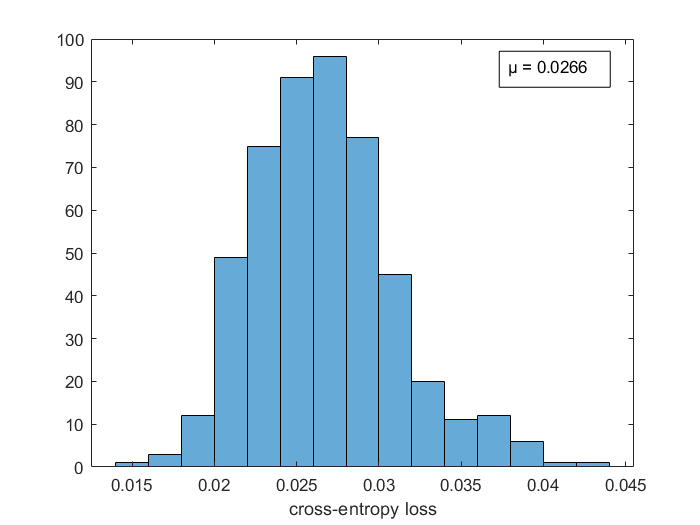
\includegraphics[width=\textwidth]{figures/CLASS/ce_hist_500.png}
  \end{subfigure}
  ~
  \begin{subfigure}[b]{0.48\textwidth}
    \centering
    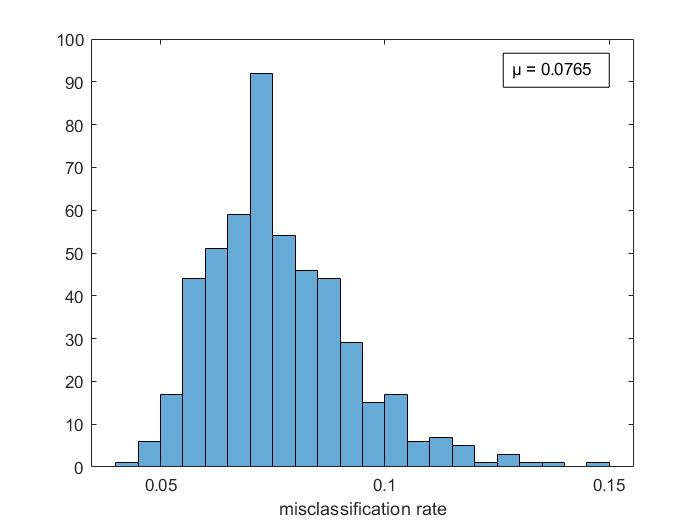
\includegraphics[width=\textwidth]{figures/CLASS/misclassification_hist_500.png}
  \end{subfigure}
  \caption{CE and Error rate for the FHR pattern network}
  \label{fig:CLASS_HIST}
\end{figure}

\begin{figure}[htb]
  \centering
  \begin{subfigure}[b]{0.48\textwidth}
    \centering
    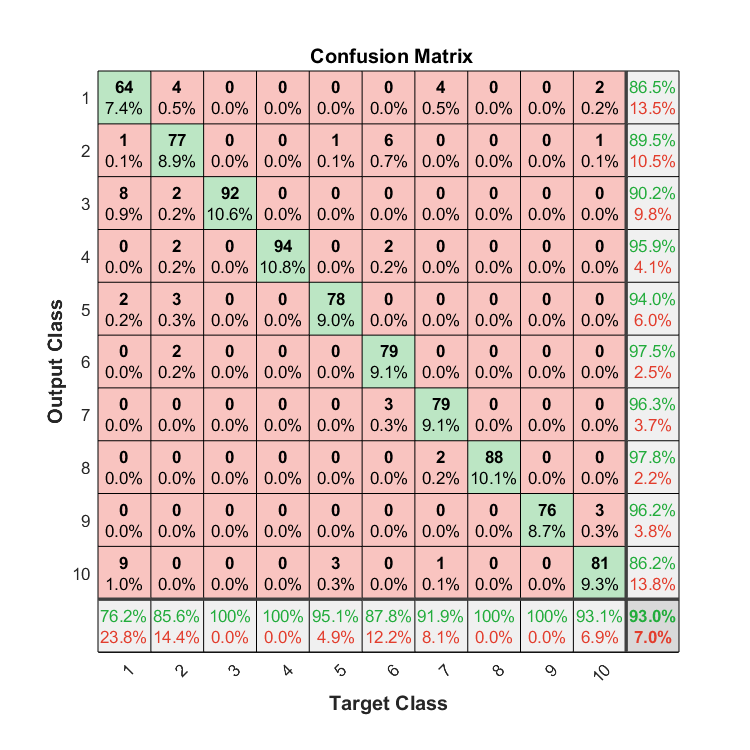
\includegraphics[width=\textwidth]{figures/CLASS/avg_conf_matrix.png}
  \end{subfigure}
  ~
  \begin{subfigure}[b]{0.48\textwidth}
    \centering
    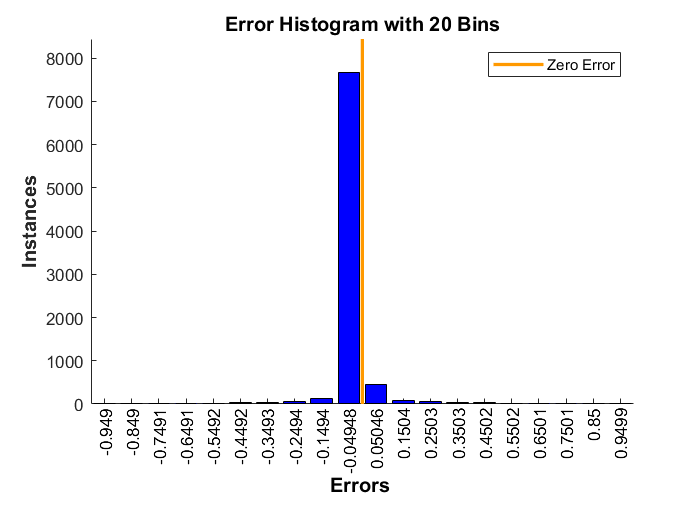
\includegraphics[width=\textwidth]{figures/CLASS/avg_err_hist.png}
  \end{subfigure}
  \caption{Performance of the average FHR pattern model}
  \label{fig:CLASS_AVG}
\end{figure}


\begin{figure}[htb]
  \centering
  \begin{subfigure}[b]{0.48\textwidth}
    \centering
    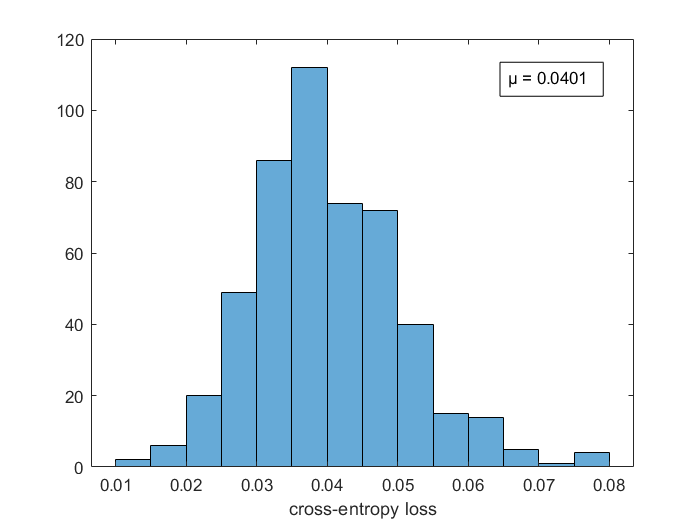
\includegraphics[width=\textwidth]{figures/NSP/ce_histogram_500.png}
  \end{subfigure}
  ~
  \begin{subfigure}[b]{0.48\textwidth}
    \centering
    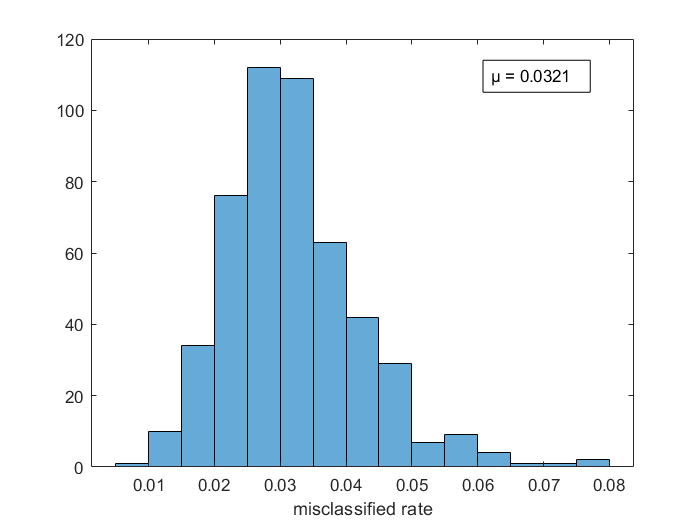
\includegraphics[width=\textwidth]{figures/NSP/misclasified_histogram_500.png}
  \end{subfigure}
  \caption{CE and Error rate for the NSP network}
  \label{fig:NSP_HIST}
\end{figure}

\begin{figure}[htb]
  \centering
  \begin{subfigure}[b]{0.48\textwidth}
    \centering
    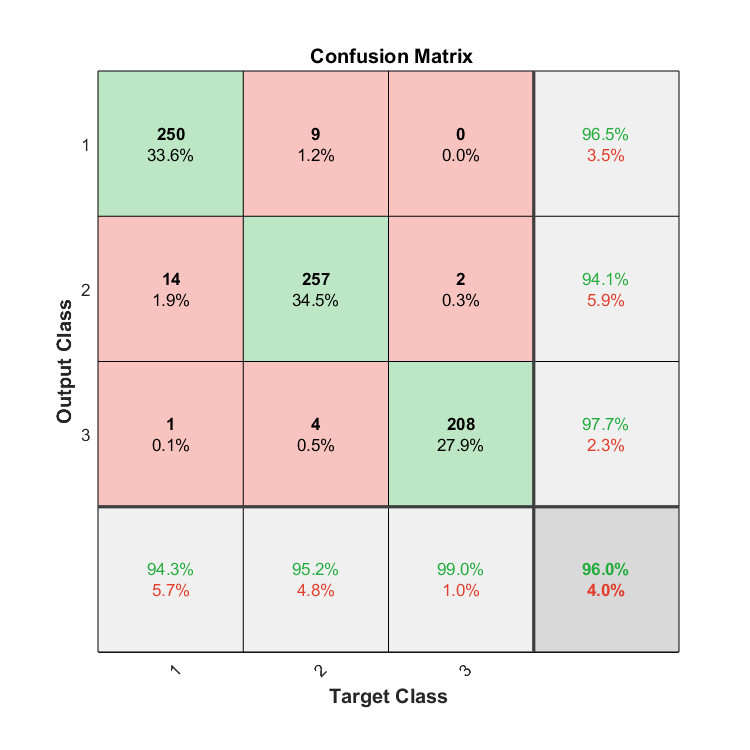
\includegraphics[width=\textwidth]{figures/NSP/avg_conf_matrix.png}
  \end{subfigure}
  ~
  \begin{subfigure}[b]{0.48\textwidth}
    \centering
    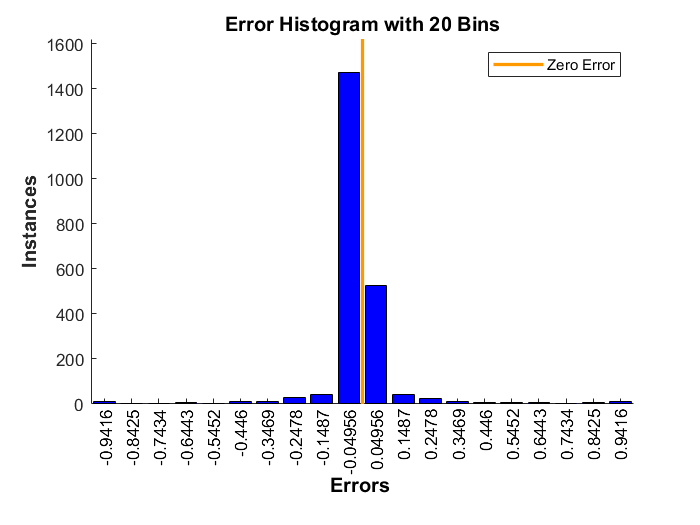
\includegraphics[width=\textwidth]{figures/NSP/avg_err_hist.png}
  \end{subfigure}
  \caption{Performance of the average NSP model}
  \label{fig:NSP_AVG}
\end{figure}


\section{[20 marks] Further application}
\label{sec:further}
In the previous sections you used a neural network to convert cardiotocogram features into a diagnosis. Another tool for detection and diagnosis of fetal abnormalities is the ultrasound scan, that produces an image of the a section through the fetus. Interpreting fetal scans is a highly complex task which require years of training. Assume the availability of a large number of fetal scan images, both normal and with some abnormality, and labelled to indicate different types of abnormalities. The task is for a neural network to process new ultrasound images, and to indicate which images needed further investigation. This section should discuss the issues you would need to consider in relation to:
\begin{outline}
  \1 selection of an architecture
  \1 construction of the network
  \1 use of data for training
  \1 evaluation of the network
\end{outline}

%TODO: Read up on Convolutional neural networks

\end{document}
